\documentclass{article} % For LaTeX2e
\usepackage{nips13submit_e,times}
\usepackage{hyperref}
\usepackage{url}
\usepackage{graphicx}
\usepackage{caption}
\usepackage{subcaption}
%\documentstyle[nips13submit_09,times,art10]{article} % For LaTeX 2.09

\usepackage{amsmath}
\usepackage{algorithm}
\usepackage{algpseudocode}

\title{House Prices Prediction using Machine Learning}


\author{
Gang Wu\\
\texttt{gangwu@stanford.edu} \\
}

% The \author macro works with any number of authors. There are two commands
% used to separate the names and addresses of multiple authors: \And and \AND.
%
% Using \And between authors leaves it to \LaTeX{} to determine where to break
% the lines. Using \AND forces a linebreak at that point. So, if \LaTeX{}
% puts 3 of 4 authors names on the first line, and the last on the second
% line, try using \AND instead of \And before the third author name.

\newcommand{\fix}{\marginpar{FIX}}
\newcommand{\new}{\marginpar{NEW}}

\nipsfinalcopy % Uncomment for camera-ready version

\begin{document}


\maketitle

\begin{abstract}   
	Recent breakthroughs on CNN and RNN have significantly improved
	the performance of many computer vision algorithms and machine comprehension 
	algorithm. It has become a very active research area. 
	In this project, I work on the house price prediction.
	Given the house image,
	a short description and other numerical features of the house,
	the goal is to predict how much will it sell.
	In particular, pretrained CNN and RNN are combined together to extract features from the 
	house image and description. 
	A linear layer is then used to combine all the extracted features together
	with the numerical features and make the prediction.
	A baseline implementation based on linear regression is also developed for 
	comparing with the neural network approach.
	
\end{abstract}

\section{Introduction}

Real estate always been a hot topic, especially in the recent years.
In this project, I work on a practical problem on this topic:
given a set of features (e.g. location, build year, etc.), an image
and a short description for a house,
how much will it sell?
The answer to this question will attract great interest to house buyers and sellers.
%I will explore various machine learning techniques in this project to help answer this question.

Recent breakthroughs with convolutional neural networks (CNN)
and recurrent neural network (RNN) have significantly improved the performance for both the image classification tasks \cite{simonyan2014very} and machine comprehension tasks \cite{cho2014learning}. 
In particular, deeper neural
networks have shown to be able to integrate more varieties 
of features and thus gaining better performance. 
As the network gets deeper and deeper, approaches such as residual networks are proposed in order to resolve the vanishing exploding gradients problem \cite{szegedy2016rethinking}
\cite{he2016deep} during training on CNN.
Also, different attention techniques such as bi-directional attention flow \cite{seo2016bidirectional}
and self-attention scheme \cite{wang2017gated} are proposed to improve the performance of RNN.

In this work, I explore the idea of combining both image recognition and machine comprehension together with the numerical features for the task of housing price prediction.
The dataset is scrapped from online websites which contain 
the pictures of the house, a short description of the house
and a set of features such as square footage, school scores, year built, etc.
The state-of-art pretrained image recognition network ResNet \cite{he2016deep}
is used to convert the housing images into feature vectors.
For the house description, Glove \cite{pennington2014glove} and LSTM \cite{hochreiter1997long} 
are used as word embedding and RNN for converting the descriptions into feature vectors.
All features are combined together though a linear layer for the final
prediction of the estimated housing price.

The reminder of this report is organized as follows:
In Section 2, I define the housing price prediction problem.
In Section 3, I discuss the related works on image recognition and machine comprehension.
The proposed neural network model is presented in Section 4.
In Section 5, the dataset will be presented and analyzed.
Finally, the experiments and conclusion are presented in Section 6 and 7.

\section{Problem Definition}

\subsection{Input \& Output}

The input to my problem would be a set of feature values for a house,
such as `year built', `lot size', `living room size', `school district', etc.
Also an image and a short description of the house.
The output is the predicted sale price.

%As a concrete example, below is a simplified set of feature values for a house as an input:
%
%$['year\_built', 'lot\_size', 'livingroom\_size', 'school\_score'] = [2001, 3000, 800, 9]$
%
%The output would be its sale price in USD: $650000$.

\subsection{Evaluation Metric}

For this work, I use Root-Mean-Squared-Error (RMSE) to evaluate the model \cite{rmse}:
\begin{equation*}
	RMSE = \sqrt{\frac{\sum_{t=1}^{T}(y_t' - y_t)}{T}}
\end{equation*}

Here, $y_t'$ denotes the logarithm of predicted house price 
and $y_t$ denotes the logarithm of real house price.
Taking logs will help make sure that errors in predicting expensive houses 
and cheap houses affect the result equally.

\section{Related Work}

\textbf{CNN based image recognition}.
Image recognition has been a very active research area
and there are many previous works on this topic.
In \cite{simonyan2014very},
the authors propose the VGG network, which stacks many small filters into deep layers.
It has the benefits of having the same effective receptive filed as the larger filters,
while be able to contain more non-linearities and uses fewer parameters.
In \cite{he2016deep}, ResNet are proposed which enables a much deeper network 
by leveraging the residual connections and has become the default standard for most recent applications.
There are also other proposed approaches such as the DenseNet\cite{huang2017densely},
which uses dense blocks to connect each layer to every other layer in a feedforward fashion,
and SE-ResNet\cite{hu2017squeeze} which improves ResNet by adding a feature recalibration module to adaptively reweight the feature maps.

\textbf{RNN based machine comprehension}.
Machine comprehension is the ability for the machine to read text and then perform predictions related to the text.
It is a challenging topic while has become a very hot research field nowadays, 
due to the recent breakthrough in deep learning neural networks.
Besides the very famous long short-term memory (LSTM) \cite{hochreiter1997long} 
and gated recurrent units (GRU) \cite{cho2014learning}
Recently, techniques based on the idea of attention has shown large performance improvement on the machine comprehension systems.
The basic idea of attention is to make the system focus on a particular part of the context during the decoding process. 
Therefore, it can overcome the bottleneck issue encountered on the recurrent neural network \cite{cho2014learning}.
In addition to different attention schemes, various other approaches have been proposed to improve the machine comprehension system. In \cite{chen2017reading}, the authors show the performance can be greatly improved by adding extra input features such as exact match or POS. In \cite{wang2016machine}, the authors have proposed an answer pointer network to better predict the starting and ending probabilistic distribution of the answer.

\section{Proposed Model}

An overview of the proposed model is shown in Figure 5.
CNN and MAC is used to extract a global feature vector from the graph.
Glove word embedding and Bi-directional LSTM is used to encode the house description.
Finally, all the extracted vectors are combined together with
the numerical features to produce the final predicted score.

\begin{figure}[h]
	\begin{center}
		%\fbox{\rule{0pt}{2in} \rule{0.9\linewidth}{0pt}}
		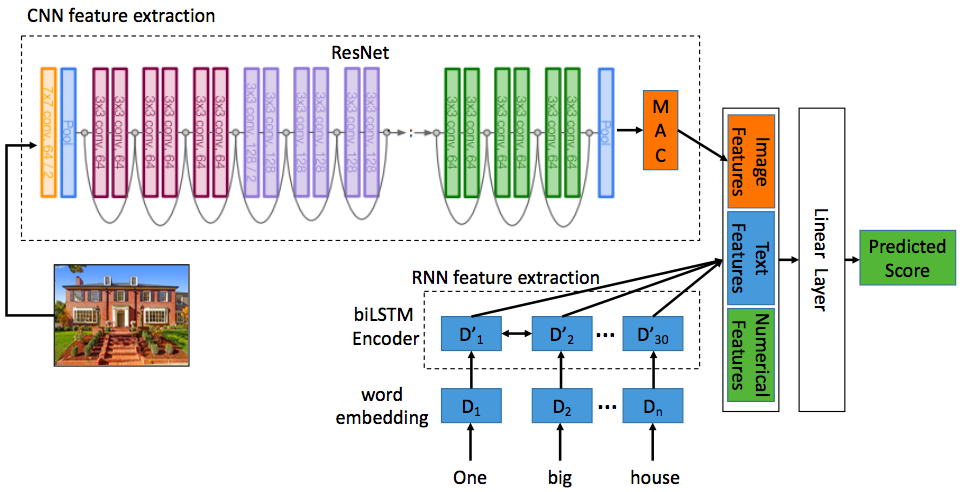
\includegraphics[width=1.0\linewidth]{fig/model.png}
	\end{center}
	\caption{The proposed model.}
\end{figure}

\subsection{CNN Feature Extraction}

\subsection{Fine-tuning CNN}

The pretrained ResNet\cite{he2016deep} is used as the CNN in the proposed model.
The dimension of the average pooling layer in the CNN network needs to be adjusted
in order to train images which have resolution different from the default.
For the ResNet implemented in PyTorch, it has a 7x7 average pooling layer
to transfer the 7x7 spacial dimension of conv5 layer to spacial 1x1 dimension
and the expected input image size is 224x224.
To make it work for other input image size, I changed the average pooling layer sized to be INPUT\_SIZE/7.

\subsection{Maximum Activation of Convolutions}

Assuming the activation of conv layer is a 3D tensor $\chi$
which contains a set of 2D tensors $\chi_i, i = 1...K$
(assuming the conv layer has K channels).
For each $\chi_i$, its valid spacial locations are denoted by $\delta$
and $\chi_i(p)$ is the activation at a particular position $p \in \delta$.
Then, we can define the maximum activation of convolution (MAC) as follows\cite{salvador2016faster}:
\begin{equation*}
\textbf{f}_{\delta} = [f_{\delta, 1} ... f_{\delta, 1} ... f_{\delta, K}]^T, with f_{\delta, i} = max_{p\in \delta}\chi_i(p)
\end{equation*}

MAC extracts one scalar value per channel and therefore transforms
the activation of conv layer into a feature vector with dimension $K$.
After training, each channel of the activation could corresponds to
a patch or a particular character of the image.
Therefore, the extracted feature vector could serve as a global 
descriptor and represents key information of the image in a compact manner.

\subsection{Bi-directional LSTM Encoder}

The input house description is first transferred to word embeddings
using pretrained Glove \cite{pennington2014glove},
it is then feed into the bi-directional LSTM for the context encoding.
By allowing the gradient to flow in both directions,
the encoding can be more context aware.

After the encoding, the hidden layers are combined together using
element-wise mean of all hidden states to get the text features.
This is better than just using the final hidden states,
as gradient can easily flow back to each stage of the sentence.

\subsection{Fully Connected Layer}

The global features extracted by CNN and the RNN encoding vectors
are concatenated together with the numerical features and feed into a fully connected layer.
The score is calculated using RMSE as shown in Section 2.2.

\section{Dataset}

Housing data is extracted from the online website through web scrapping.
There are data for a total amount of 5217 houses in the 
Portland downtown area.
It is limited to single family houses sold within the past one year.


\subsection{Numerical Features}

Figure 2 shows the histogram of the sale price among the whole dataset.
We can see the mean value of the sale price is 437K USD
with a standard deviation of 182K USD.

\begin{figure}[h]
	\begin{center}
		%\fbox{\rule{0pt}{2in} \rule{0.9\linewidth}{0pt}}
		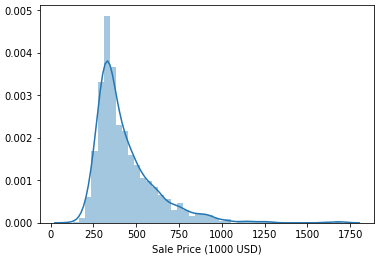
\includegraphics[width=0.5\linewidth]{fig/sale_price.png}
	\end{center}
	\caption{Histogram of sale price.}
	\label{fig:long}
	\label{fig:onecol}
\end{figure}

Besides `SoldPrice', other useful numerical features scrapped are:

`ZipCode', `Beds', `Bath', `SquareFeet', `YearBuilt', `Stories', `LotSize'

There are also school scores rated from 1 to 10 for the elementary school, middle school and high school
of the corresponding school district.
In addition, Redfin provides a `Walk Score', `Transit Score', `Bike Score' from 1 to 100
for describing the transportation convenience of the house.

Figure 1 below shows a heat map about the correlation between different features and the sold price.
It can be seen that the square footage is the strongest indicator of the sell price among all the features.
Next would be the school scores.
The built year and zip code are shown as the weakest (or even negative) indicator of the sell price.

\begin{figure}[H]
	\begin{center}
		%\fbox{\rule{0pt}{2in} \rule{0.9\linewidth}{0pt}}
		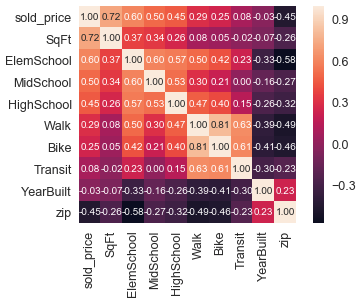
\includegraphics[width=0.5\linewidth]{fig/heatmap.png}
	\end{center}
	\caption{Heat map showing correlation between different features and the sold price.}
\end{figure}

Figure 4 below provides a more detailed look for the relation between sold price, school score and square footage of the house.
It can be seen that the elementary school score and square footage 
all has a linear relationship with the sold price.

\begin{figure}[H]
	\begin{center}
		%\fbox{\rule{0pt}{2in} \rule{0.9\linewidth}{0pt}}
		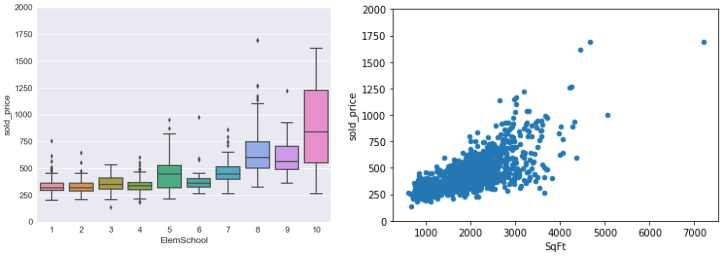
\includegraphics[width=0.85\linewidth]{fig/cmp.png}
	\end{center}
	\caption{(a) Relationship between elementary school score and sold price. (b) Relationship between square footage and sold price.}
\end{figure}

Figure 5 shows the box plot for the relationship between the build year and sale price.
However, we cannot see a clear relationship between these two values.
Both newly built houses and old houses can have high prices.

\begin{figure}[H]
	\begin{center}
		%\fbox{\rule{0pt}{2in} \rule{0.9\linewidth}{0pt}}
		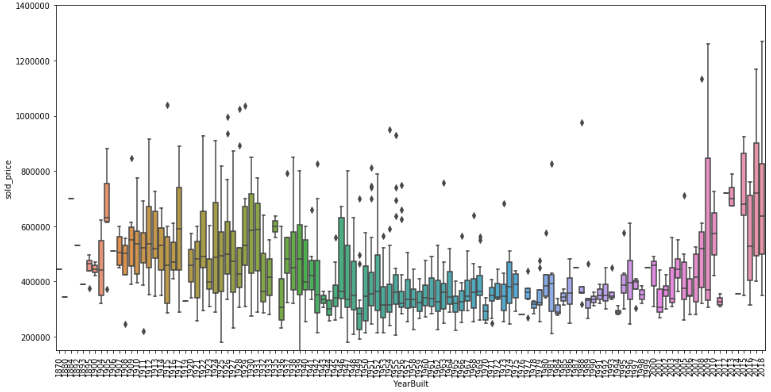
\includegraphics[width=0.8\linewidth]{fig/build_year.png}
	\end{center}
	\caption{Relationship between build year and sale price.}
	\label{fig:long}
	\label{fig:onecol}
\end{figure}

\subsection{Short Description}

The short description is scrapped from a commenting section on the website.
Section 5.2.1 shows the description for the cheapest house (\$132K) in the dataset,
while Section 5.2.2 shows the one for the most expensive house (\$1694K).
As shown in the description, the cheap house only has 1 bedroom and 1 bathroom.
It also needs further upgrades \& repairs.
However, the expensive house is specially designed with a lot of nice features.

\subsubsection{Description of the cheapest house in the dataset}

``Opportunity awaits in this 1 bedroom 1 bathroom dwelling. The home offers the chance to earn rental income. It will take some upgrades and repairs to ready this home for renters but it could be worth the time. Come and see if this will be your new investment."

\subsubsection{Description of the most expensive house in the dataset}

``Stately Georgian Colonial home designed by Roscoe Hemenway is unveiled as a complete restoration by Portland Houseworks. Grand foyer w/curved staircase, glass hanging chandelier \& cstm wainscotting.Mltpl entertaining spaces w/open great rm kitchen anchored by quartz island, formal dining, builtins \& white oak floors. Gourmet kitchen w/Walker Zanger tile backsplsh, large Wolf app \& sub-zero refrig. Wet bar, kitchenette, dual wine refri."

\subsection{Images}

A front view image is extracted for each house.
Figure 3 shows the images for the 6 cheapest houses among the entire dataset
and Figure 4 shows the 6 most expensive houses.
Comparing the two sets, it is not hard to find the difference between them:
expensive houses tend to be more clean, tidy and most of them 
come with big green grass lands.
One the country, cheap houses are small, dirty and
the grass lands are scattered or yellow.

\begin{figure}[h]
	\begin{center}
		%\fbox{\rule{0pt}{2in} \rule{0.9\linewidth}{0pt}}
		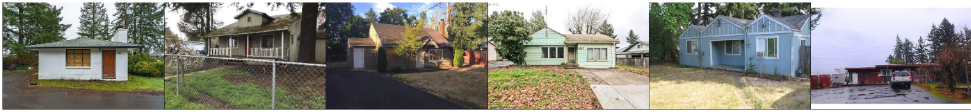
\includegraphics[width=1\linewidth]{fig/cheap_img.png}
	\end{center}
	\caption{The 6 cheapest houses among the entire dataset.}
\end{figure}

\begin{figure}[h]
	\begin{center}
		%\fbox{\rule{0pt}{2in} \rule{0.9\linewidth}{0pt}}
		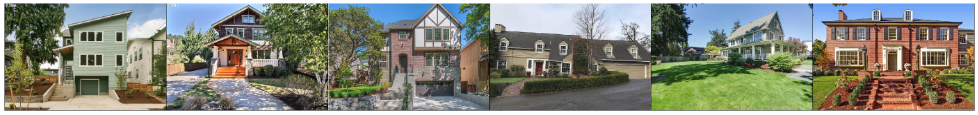
\includegraphics[width=1\linewidth]{fig/exp_img.png}
	\end{center}
	\caption{The 6 most expensive houses among the entire dataset.}
\end{figure}

\section{Experiments}

The model is implemented using PyTorch.
The training is performed on Nvidia GTX 1080 Ti with 11GB memory
and 6 Core i7 CPU with 32 GB memory.
%Adam optimizer is used with the learning rate $1e-3$.

\subsection{Preprocessing}

Data with missing image or description fields are pruned out.
The dataset is splited into two parts: 70\% on the $training\_set$ for training
and 30\% on the $dev\_set$ for cross validation.
The images are resized to 224x224 and normalized.
For the house description, only alphabet and numerical characters are kept.
All the characters are transferred to lower case.
The description size is limited to 100 words, 
by truncating longer sentences and padding short sentences.
%I also extracted all the 37 numerical features while ignoring the
%rest 43 categorical features for a simple baseline implementation.
%The missing feature values are filled using the median value of the feature.
%This ends up with the $training\_set$ dimension $(1022, 37)$ and $dev\_set$ dimension $(438, 37)$.

\subsection{Baseline Implementation}

Figure 2 (a) shows the linear regression results \cite{lr} on $training\_set$ and $dev\_set$
and Figure 2 (b) shows the results of XGBoost\cite{xgboost}.
To note that, the linear regression only considers the numerical features,
while ignores the house images \& descriptions.
The corresponding RMSE and $R^2$ scores are shown in Table 1.
From the result, we can see the XGBoost model helps remove the few outliers in the $training\_set$.
However, the results on the $dev\_set$ is not improved which shows the XGBoost model is overfitting.

\begin{figure}[h]
	\begin{center}
		%\fbox{\rule{0pt}{2in} \rule{0.9\linewidth}{0pt}}
		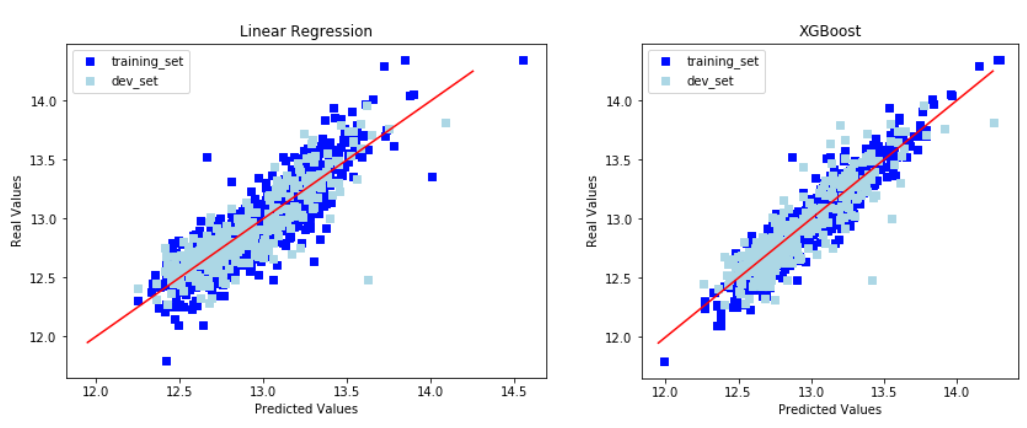
\includegraphics[width=1\linewidth]{fig/exp.png}
	\end{center}
	\caption{(a) Linear regression. (b) XGBoost.}
	\label{fig:long}
	\label{fig:onecol}
\end{figure}

\begin{table*}[h]
	\begin{center}
		\begin{tabular}{|l|cc|cc|}
			\hline
			 Method &
			TrainSet-$RMSE$ &
			DevSet-$RMSE$ &
			TrainSet-$R^2$ &
			DevSet-$R^2$ \\
			\hline
			LR & 0.176 & 0.170 & 0.755 & 0.723 \\
			\hline
			XGB & 0.159 & 0.171 & 0.800 & 0.720 \\
			\hline
		\end{tabular}
	\end{center}
	\caption{RMSE and $R^2$ score with linear regression and XGBoost.}
\end{table*}

\subsection{Regression with ResNet, LSTM and Numerical Features}

Adam optimizer is used during training with learning rate of $1e-3$.
The batch size is set to be 64 during training and 128 during evaluation.

For the details of ResNet,
the input image size is $64 \times 3 \times 224 \times 224$ 
(here I assume the batch size during training).
After feeding the images to ResNet50,
I get its Conv3 layer with size $64 \times 512 \times 28 \times 28$.
Then I preform maximum activation pooling on the Conv3 layer
and ends up with the image feature vector of size $64 \times 512$.

For LSTM, since I limit the text length to be 100 and using glove.6B.50d,
the input embeding size to the RNN is  $64 \times 100 \times 50$.
 Also, I choose the hidden layer size to be $50$,
 therefore, I got the output also as a vector with size $64 \times 100 \times 50$.
 Then I perform averaging on the $100$ hidden vectors and ends up with the text
 feature vector of size $64 \times 50$.
 
 For numerical features,
 ``squre footage", ``elemSchool score", ``midSchool score", ``highSchool score"
 ``walk score", ``transit score" and ``bike score" are used.
 All of them are normalized at each feature.
 Combining the numerical features with the image and text features,
 I get a feature vector of size $64 \times 569$.
 The combined feature vector is then feed into the linear layer to get the final prediction score.

It takes about 30 seconds to load the glove vector, 12 seconds for pytorch to build the model
and about 5 minutes to train each full epoch with GPU.
The comparision results are shown in Table 2.
It can be seen that the neural network based approach 
can greatly improve the proformance from the baseline linear regression model.
Also, the 50 dimention glove vector did not show too much performance improvement
from just using the basic ResNet + NumFeatures.
However, the results get improved a lot after I try the 300 dimention glove vector.
The dev results also get improved further after I adding regulariztion on the LSTM.

\begin{table}
	\label{sample-table2}
	\begin{center}
		\begin{tabular}{|c|cc|}
			\hline
			\multicolumn{1}{|c|}{}  &\multicolumn{1}{c}{\bf Train RMSE} &\multicolumn{1}{c|}{\bf Dev RMSE} \\ 
			\hline
			baseline                                                   &0.176 &0.170\\
			ResNet + NumFeatures           					&0.107 &0.121\\
			ResNet + biLSTM + NumFeatures           &0.109 &0.110\\	
			with glove840B300d             &0.091 &0.102\\
			with regularization             	&0.090 &0.097\\
			\hline
		\end{tabular}
	\end{center}
	\caption{Comparing the results of adding different components.}
\end{table}

%\begin{figure}[h]
%	\begin{center}
%		%\fbox{\rule{0pt}{2in} \rule{0.9\linewidth}{0pt}}
%		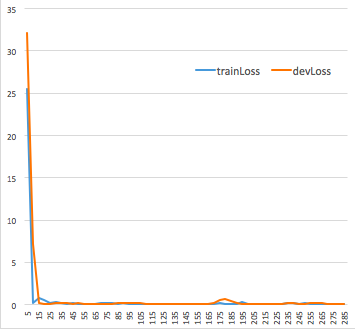
\includegraphics[width=0.45\linewidth]{fig/loss.png}
%	\end{center}
%	\caption{Train and dev loss on the dataset.}
%	\label{fig:long}
%	\label{fig:onecol}
%\end{figure}

%\section{Error Analysis}


\section{Conclusion \& Future Work}

In this project, I developed a neural network model to predict the housing price
based on the house images, descriptions and some numerical features.
By combining CNN with RNN, the prediction performance get improved on the linear model,
as the model can leverage both the information extracted from images and texts.

There are still many works can be done on this project:
one thing is to do the fine tuning and analysis of both the ResNet and the bi-LSTM. 
Also, ensembling technique can be used. Different architectures can be tried for CNN (e.g DenseNet, SE-ResNet) and RNN (e.g. GRU), then be ensembled together to improve the performance.


{\small
	%\bibliographystyle{ieee}
	\bibliographystyle{unsrt}
	\bibliography{nips2013}
}



\end{document}
